\providecommand{\topdir}{..}
\documentclass[../main.tex]{subfiles}

\newacronym[description={Scattering measured at very undeflected angles (small angles). Can be conducted using electrons, radiation and neutrons}]
{glos:SAS}{SAS}{Small Angle Scattering}

\newacronym[description={X-ray version of SAS}, parent=glos:SAS]
{glos:SAXS}{SAXS}{Small Angle X-ray Scattering}

\newacronym[description={Scattering measured at larger deflected angles (wide angles). Can be conducted using electrons, radiation and neutrons}]
{glos:WAS}{WAS}{Wide Angle Scattering}

\newacronym[description={X-ray version of WAS}, parent=glos:WAS]
{glos:WAXS}{WAXS}{Wide Angle X-ray Scattering}

\newacronym[description=The constructive and destructive inteference of scatterers passing through a periodic material results in diffraction peaks.]
{glos:XRD}{XRD}{X-ray Diffraction}

\newacronym[description=The use of small grasing angles to measures small momentum changes.]
{glos:GI}{GI}{Grasing Incidence}

\newglossaryentry{glos:ewald}{
	name=Ewald Sphere,
	description={The curved slice }
}

\begin{document}
	\chapter{Small/Wide-Angle-Xray-Scattering}\label{chap:05-saxs-waxs}
		One of many \gls{glos:SAS} methods (which also include the use of electrons and neutrons) is \gls{glos:SAXS}.
		
		\begin{figure}[H]
			\centering
			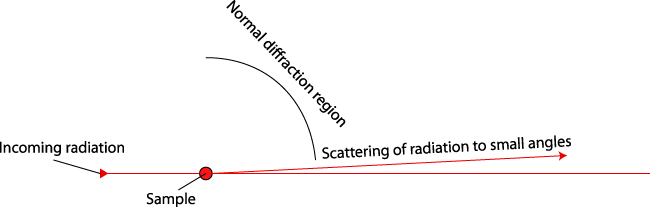
\includegraphics[width=0.5\textwidth]{resources/ch5/cm440881f1_hr}
			\caption{The \acrfull{glos:SAXS} method measures radiation scattered at small angles, compared to the typical diffraction angles utilised in \gls{glos:XRD}.}
			\label{fig:ch5-SAXS}
		\end{figure}
		
		The alternative to \gls{glos:SAS} is \gls{glos:WAS}. Wide angle scattering occurs when 
		
		\section{Detector positioning}
			\subsection{Small angle}
				Small angle X-ray scattering (\gls{glos:SAXS}) measurements generally refer to small $q$ resolution accessible by the measurement geometry. Typical incident - deflected $2\theta$ angles are from \qtyrange{0}{5}{\degree}. This allows the resolution of large structures, from \SI{0.3}{\angstrom} to \SI{50}{\nano\metre} in size (i.e. $1/500 = $ \SI{0.002}{\per\angstrom}). For example, the Australian Synchrotron SAXS/WAXS beamline allows SAXS measurements with $q$ ranges between \qtyrange{0.0015}{3.0}{\per\angstrom} (approximately real spacing of \qtyrange{66}{3}{\nano\metre}). By placing a detector far away from the scattering plane (transmission) / axis (grazing incidence), the resolution in small angles is enhanced, and consequently small momentum scattering changes can be easily detected.
			
			\subsection{Wide angle}
				Wide angle X-ray scattering (\gls{glos:WAXS}) measurements generally refer to larger $q$ range accessible by the measurement geometry. Typical incident - deflected $2\theta$ angles are from \qtyrange{5}{60}{\degree}. This corresponds to features smaller than \SI{1}{\nano\metre} (i.e., $1/0.2 = $ \SI{5}{\per\angstrom}).
				For example, the Australian Synchrotron SAXS/WAXS beamline allows WAXS measurements with $q$ ranges between \qtyrange{0.6}{10.0}{\per\angstrom} (approximately real spacing of \qtyrange{2}{0.1}{\angstrom}). By placing a detector far away from the scattering plane (transmission) / axis (grazing incidence), the resolution in small angles is enhanced, and consequently small momentum scattering changes can be easily detected.
		
		\section{Measurement geometries}\label{sec:ch5-geoms}
			Two methods, Transmission (\cref{sec:ch5-geoms-transmission}) and \gls{glos:GI} (\cref{sec:ch5-geoms-grasing_incidence}) are primarily used to measure the scattering from targets.
			As the incident light has electric and magnetic field directions perpendicular to the direction of propagation, these geometries pertain to different knowledge about the sample, because of the relative polymer orientations.
			\subsection{Transmission}\label{sec:ch5-geoms-transmission}
				Transmission geometry places the sample plane perpendicular to the beam direction. Therefore, the electric field \textit{polarisation} of the beam is either parallel or perpendicular to polymer orientation. This can cause strong coupling to particular bonding directions, such as along a polymer's backbone where scattering is uniform throughout the sample. If the film has been created via \gls{glos:rubbing} or \gls{glos:blade-coating}, then the 
						
			\subsection{Grazing Incidence}\label{sec:ch5-geoms-grasing_incidence}
				Grazing incidence (\gls{glos:GI}) geometry places the sample plane parallel to the beam direction. Hence, polymer chains are either parallel to the beam direction or perpendicular in plane.
				Distinguished from transmission geometry, the measurement is sensitive to typically the first few nano-meters of the film thickness. Additionally, out-of-plane scattering introduces a new measurement directionality. Consequently, \gls{glos:GI} measurements reveal orbital alignment to the out-of-plane direction, distinguishing between "Edge on" or "Face on" orientations, which may or may not be different to the bulk orientations.
				
				\begin{figure}[H]
					\centering
					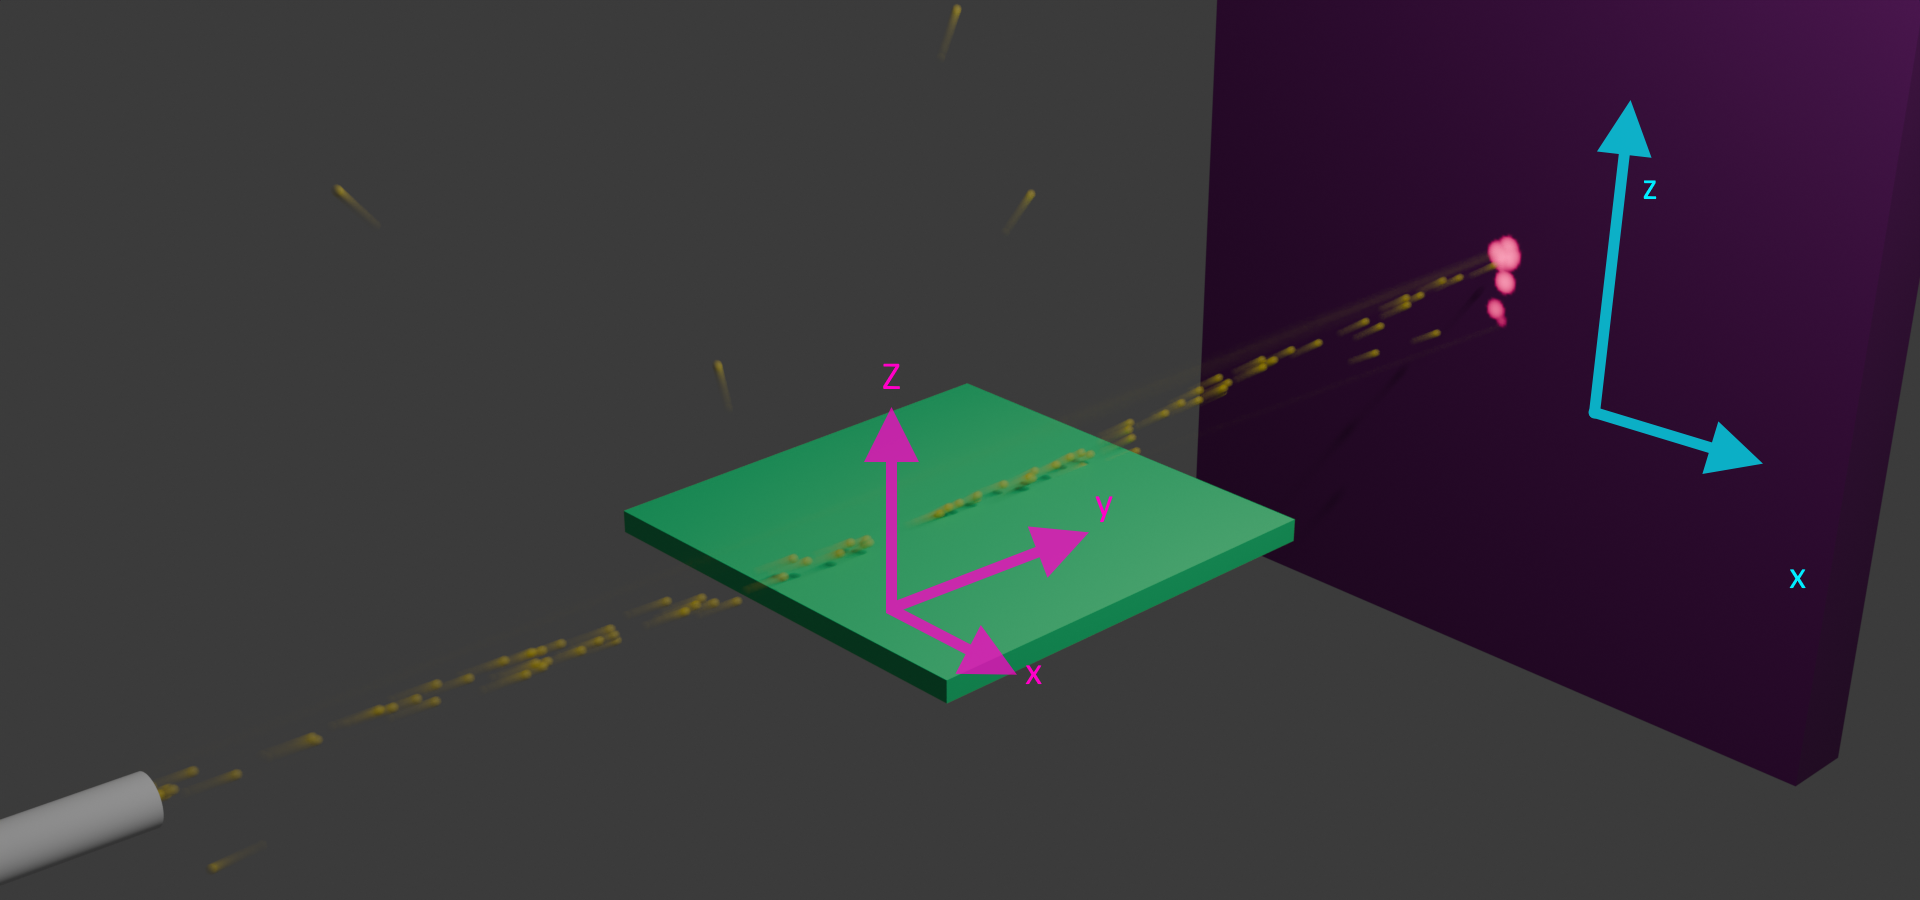
\includegraphics[width=0.8\textwidth]{resources/ch5/GrasingIncidence-0052_labelled}
					\caption{}
					\label{fig:ch5-SAXS-GI}
				\end{figure}
				
				\subsubsection{The Ewald Sphere}\label{sec:ch5-geoms-grasing_incidence-ewald}
					When incident light scatters from the a periodic structure, diffraction peaks result from the constructive and destructive interference  due to the path length of the spacing. Therefore diffraction appears as a Fourier signal (a frequency) that corresponds to a particular spacing - this is what we measure in $q$ space on our detector.
					When performing scattering at grazing incidence, the sample scatters in the following directions (and corresponding reciprocal space):
					\begin{itemize}
						\item $z$, $q_z$ - Normal to the film
						\item $y$, $q_y$ - Along the beam
						\item $x$, $q_x$ - Perpendicular to the beam and normal.
					\end{itemize}
					
					The reciprocal lattice is 3D; The detector cuts a slice of this space to analyse peaks, 
					For small $q$ angles, such as in SAXS, the curvature of the Ewald sphere can be approximated as negligible.
					
					At wide angles (WAXS), the curvature of the reciprocal space becomes really important, as the detector pixels are no longer just probing ($q_x$, $q_z$) but ($q_x$, $q_y$, $q_z$).
				
				
		\section{Application to organic semiconductors}

\ifSubfilesClassLoaded{
	\printbibliography{}
	\printglossaries
}{} % we have no 'else' action
	
\end{document}